\setcounter{ExampleCounter}{1}
There's an old legend about the inventor of chess, who, when he was asked by the ruler what reward he desired for his invention, told the ruler to simply pay him in rice.  In fact, he said, the ruler could simply place one grain of rice on the first square of a chessboard, followed by two grains of rice on the next square, and so on, doubling each time.  Surprised by how little the inventor requested, the ruler agreed, and began adding rice to the board.

\begin{center}

\includegraphics[width=0.8\textwidth]{riceboard}
\end{center}

He quickly ran into a problem, though.  By the time he reached the 21st square, he had to deliver over a million grains of rice, and by the 31st square, it was over a billion squares.  He called in his best mathematicians, and to his horror, they informed the ruler that if he kept up his side of the bargain, he would have to give the inventor a total of 18,446,774,073,709,551,615 grains of rice (about 1000 times the amount of rice harvested worldwide in a modern year).

This exposes a flaw in using exponential models for population growth.  Although doubling at every step corresponds to a 200\% growth rate, even more modest rates exhibit the same behavior when observed over a long enough time: exponential models grow without bound, and they grow faster and faster over time.

\subsection{Limited Resources}
In 1950, the world population was 2.53 billion, and it grew to 5.32 billion by 1990, 40 years later.  We can use these two data points to build an exponential model that predicts that $t$ years from 1950, the world population in billions will be \[P_t = 2.53(1.0188^t)\]

Let's test the model; let $t=55$, for example, corresponding to the year 2005.  The actual population in 2005 was 6.51 billion, and the model predicts that the population would be 7.03 billion.  Not perfect, but not terrible either.

However, what about 2015?  The model predicts 8.47 billion, and the actual population was only 7.32 billion.  In other words, the model is getting worse, and it's consistently overestimating; in 2005 the estimate was only off by half a billion, but by 2015 the error had more than doubled.  What's happening?

It turns out that the population growth rate is not constant, as the exponential model assumed.  Instead, the growth rate is slowing.  The world population grew from 1.60 billion in 1900 to 6.13 billion in 2000, so even if it grew by the same \textit{amount} (not even the same \textit{rate}, which would lead to even bigger numbers) we might naively assume that by 2100 the world population would top 11 billion.  However, the United Nations estimates that the population will top 8 billion around 2050, and then \textit{fall} back to around present-day levels by 2100.

What's going on here?  There are many factors, but one of the most fundamental is that the earth has \textbf{limited resources}.  Clearly, the population can't keep growing forever without bound; the earth cannot sustain a trillion people, for instance, given current technology, infrastructure, and access to food and water.  This leads to our conclusion:
\begin{center}
Exponential models are not good enough in the long term\\ because they don't account for limited resources.
\end{center}

\subsection{Logistic Models}
In the short term, exponential models can give decent estimates, but in the long run, they'll eventually give unsustainable results.  To account for this, we turn to \textbf{logistic models}, which do account for limited resources.

\begin{proc}{Carrying Capacity}
The \textbf{carrying capacity}, or \textbf{maximum sustainable population}, is the largest population that an environment can support.
\end{proc}

\begin{formula}{Logistic Growth}
If a population is growing in a constrained environment with carrying capacity $M$ and growth rate $r$, then the population can be described by the logistic growth model:\marginnote{The $e$ in this formula is called the \emph{natural base} (see the section on continuously compounded interest in the Financial Math chapter for more information).  The value of this number is approximately 2.7183.  To evaluate formulas with this value, look for a button on your calculator labeled \calcbutton{$e^x$}}
\[P_t = \dfrac{M}{1+\left(\dfrac{M}{P_0}-1\right)e^{-rt}}\]
\end{formula}

This model of population growth is sometimes called the \textit{Verhulst model}, after Pierre-Fran\c cois Verhulst, a Belgian mathematician who published the model in 1838\footnote{It was rediscovered and re-derived several times over the following centuries by other mathematicians studying population growth.} and used it in 1840 to predict the population of the U.S. up to 1940.  His estimate of the 1940 population of the U.S. was off by less than 1\%, a remarkable achievement.

He worked with the following data from 1790 to 1840:
\begin{center}
\begin{tabular}{c | c}
\textbf{Date} & \textbf{Population}\\
(Years AD) & (millions)\\
\hline
1790 & 3.929\\
1800 & 5.308\\
1810 & 7.240\\
1820 & 9.638\\
1830 & 12.866\\
1840 & 17.069
\end{tabular}
\end{center}

The graph below shows these data points, as well as the curve generated by a logistic model.  Note the trademark S-shape of the curve; this is typical for logistic curves---they initially look like exponential curves, but then level off as the population approaches the carrying capacity.
\begin{center}
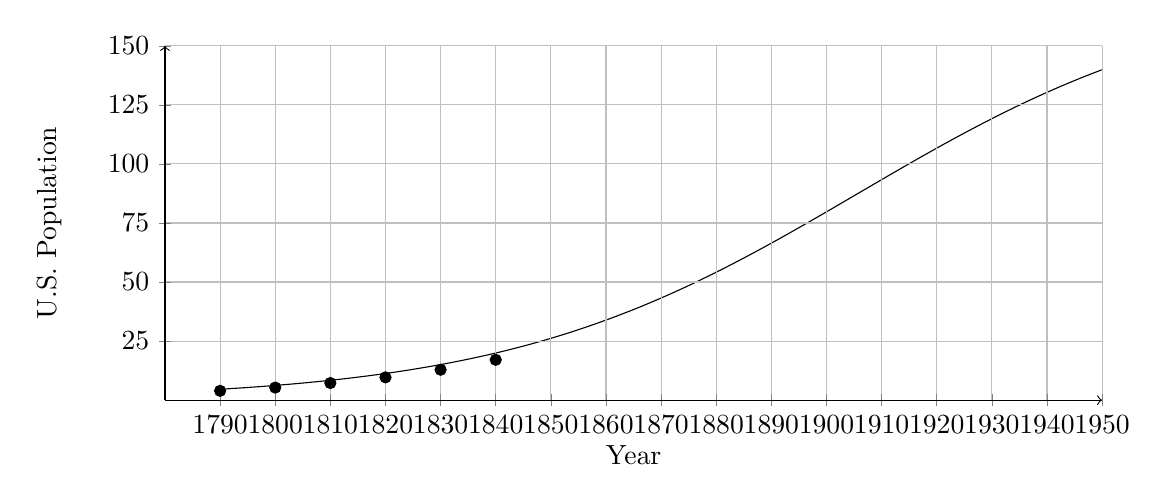
\begin{tikzpicture}
\begin{axis}[
    xmin=1780, xmax=1950,
    ymin=0, ymax=150,
    axis lines=center,
    axis on top=true,
    domain=0:1,
    x=0.07cm,
    y=0.03cm,
    xtick={1780,1790,...,1950},
    xticklabels={1780,1790,...,1950},
    ytick={0,25,...,200},
    yticklabels={0,25,...,200},
    axis lines=middle,
    axis line style={->},
    x label style={at={(axis description cs:0.5,-0.1)},anchor=north},
    y label style={at={(axis description cs:-0.1,.5)},rotate=90,anchor=south},
    xlabel={Year},
    ylabel={U.S. Population},
    grid=major
    ]
	\addplot[samples=100,domain=1790:1950] {175/(1+37.02*e^(-0.03121*(x-1790)))};
	\addplot [only marks] table {
	1790 3.929
	1800 5.308
	1810 7.24   
	1820 9.638
	1830 12.866
	1840 17.069
	};
\end{axis}
\end{tikzpicture}
\end{center}

The next graph shows the same model, but this time with data from the U.S. census filled in for the remaining years.
\begin{center}
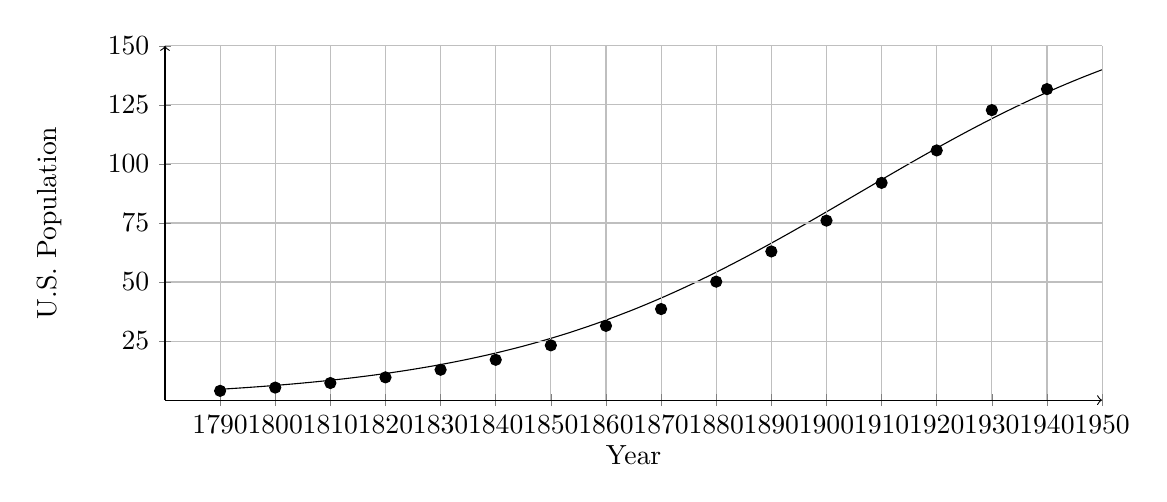
\begin{tikzpicture}
\begin{axis}[
    xmin=1780, xmax=1950,
    ymin=0, ymax=150,
    axis lines=center,
    axis on top=true,
    domain=0:1,
    x=0.07cm,
    y=0.03cm,
    xtick={1780,1790,...,1950},
    xticklabels={1780,1790,...,1950},
    ytick={0,25,...,200},
    yticklabels={0,25,...,200},
    axis lines=middle,
    axis line style={->},
    x label style={at={(axis description cs:0.5,-0.1)},anchor=north},
    y label style={at={(axis description cs:-0.1,.5)},rotate=90,anchor=south},
    xlabel={Year},
    ylabel={U.S. Population},
    grid=major
    ]
	\addplot[samples=100,domain=1790:1950] {175/(1+37.02*e^(-0.03121*(x-1790)))};
	\addplot [only marks] table {
	1790 3.929
	1800 5.308
	1810 7.24   
	1820 9.638
	1830 12.866
	1840 17.069
	1850 23.192
	1860 31.443
	1870 38.558
	1880 50.156
	1890 62.948
	1900 75.996
	1910 91.972
	1920 105.711
	1930 122.775
	1940 131.669
	};
\end{axis}
\end{tikzpicture}
\end{center}

Notice how closely the actual data tracks with the model's predictions; this is evidence of a good model, especially when we consider that the prediction was made ahead of time.  More often than you might expect, would-be experts will reach for data from the past and magically find a model that fits the data nearly perfectly, but such models tend to fail at making predictions, and they don't actually offer any insight.  A truly predictive model like this one with such accurate results is quite rare.

\begin{example}[https://www.youtube.com/watch?v=cd5xQCfLUZM&list=PLfmpjsIzhztutjEb8Pg5OBOlI1p80yVoy&index=13]{Lizard Population}
On an island that can support a population of 1000 lizards, there is currently a population of 600.  These lizards have a lot of offspring and not many natural predators, so they have a very high growth rate of 150\%.  Use a logistic model to predict the lizard population 2 years from now.

\solline
\marginnote{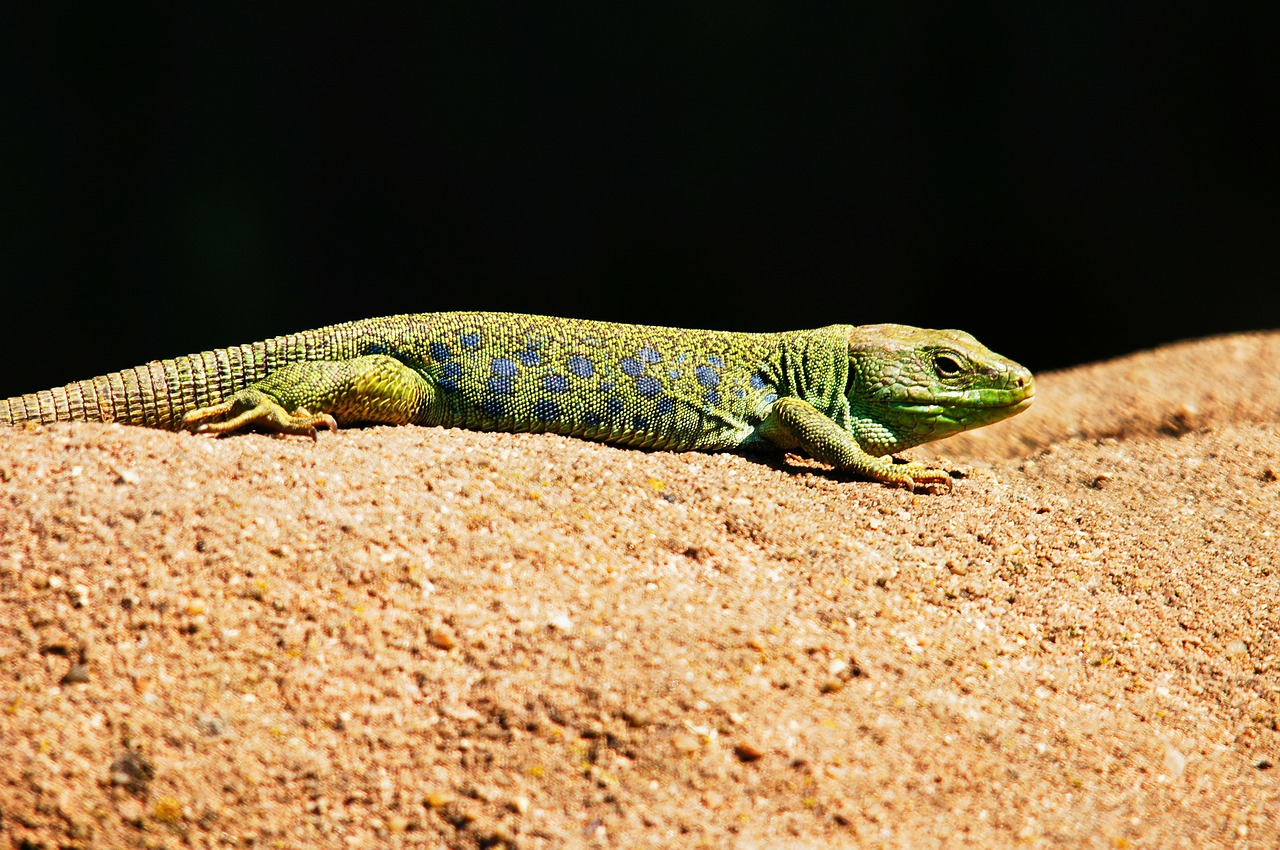
\includegraphics[scale=0.07]{Lizard1}}
Fill in the logistic model with the given information:
\begin{center}
$M=1000$, $P_0=600$, $r=1.5$
\end{center}
\begin{align*}
P_t &= \dfrac{M}{1+\left(\dfrac{M}{P_0}-1\right)e^{-rt}}\\
P_t &= \dfrac{1000}{1+\dfrac{2}{3}e^{-1.5t}}
\end{align*}

\begin{center}
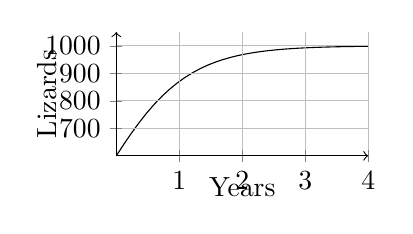
\begin{tikzpicture}
\begin{axis}[
    xmin=0, xmax=4,
    ymin=600, ymax=1050,
    axis lines=center,
    axis on top=true,
    domain=0:1,
    x=0.8cm,
    y=0.0035cm,
    xtick={0,1,...,20},
    xticklabels={0,1,...,20},
    ytick={0,100,...,1000},
    yticklabels={0,100,...,1000},
    axis lines=middle,
    axis line style={->},
    x label style={at={(axis description cs:0.5,-0.1)},anchor=north},
    y label style={at={(axis description cs:-0.2,.5)},rotate=90,anchor=south},
    xlabel={Years},
    ylabel={Lizards},
    grid=major
    ]
	\addplot[samples=100,domain=0:12] {1000/(1+(2/3)*e^(-1.5*x))};
\end{axis}
\end{tikzpicture}
\end{center}

Let $t=2$ to predict the population in 2 years:
\begin{align*}
P_2 &= \dfrac{1000}{1+\dfrac{2}{3}e^{-1.5(2)}}\\
 &= \dfrac{1000}{1.0332}
 &\approx \boxed{968 \textrm{ lizards}}
\end{align*}
The model predicts that there will be approximately 968 lizards in 2 years.
\end{example}

\begin{try}[http://hartleymath.com/versatilemath/tryit/\#/growth-models--logistic-growth-with-plants]
A field contains 20 mint plants, and the number of plants increases at a rate of 70\%, but the field can only support a maximum population of 300 plants.  Use the logistic model to predict what the population will be in three years.
\end{try}

\begin{example}[https://www.youtube.com/watch?v=mmL2H7_ynUA&list=PLfmpjsIzhztutjEb8Pg5OBOlI1p80yVoy&index=14]{Rabbit Population}
\marginnote{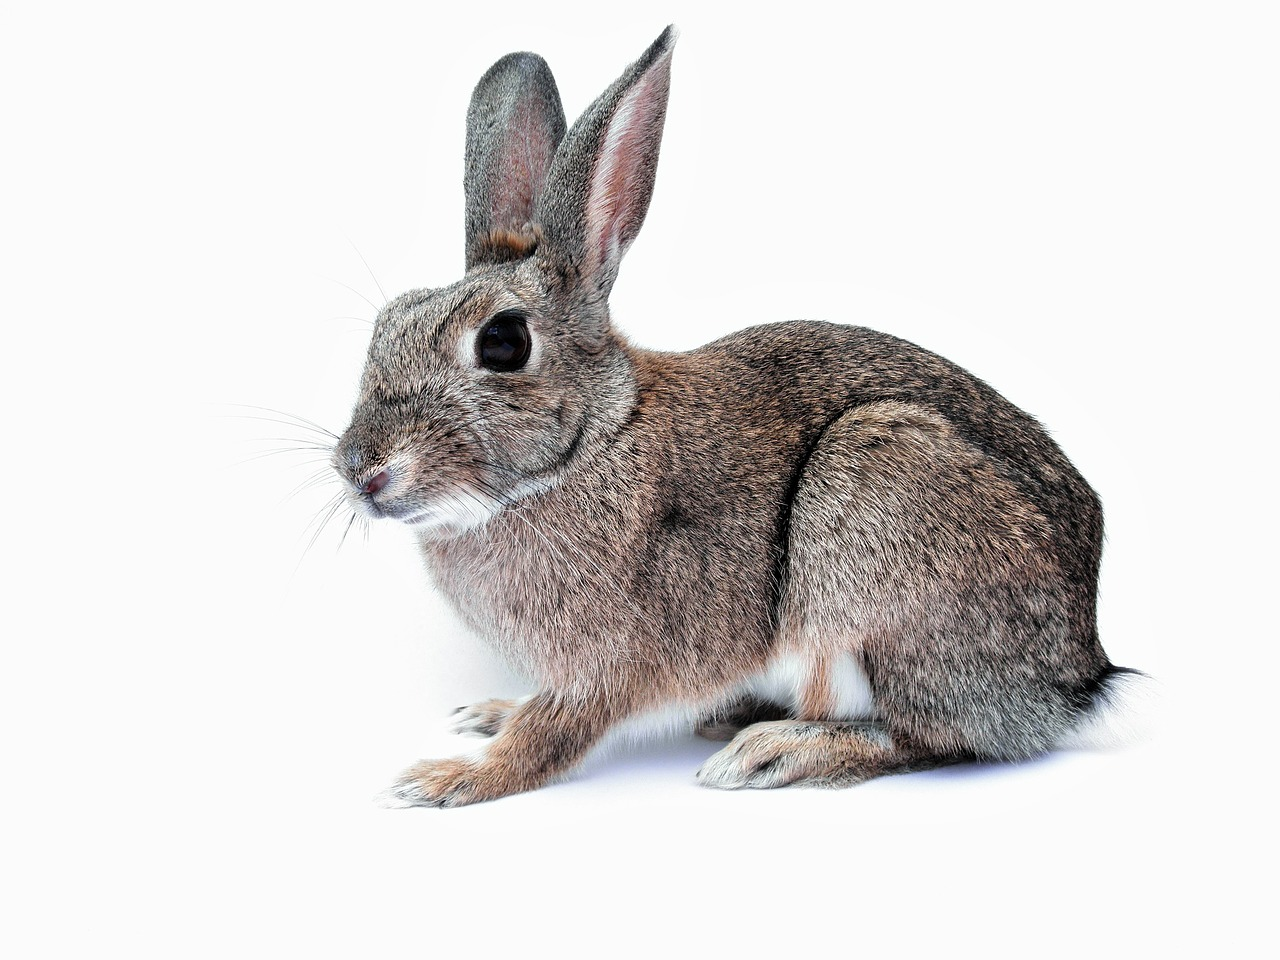
\includegraphics[scale=0.07]{Rabbit1}}
A forest is currently home to a population of 200 rabbits.  The forest is estimated to be able to sustain a population of 2000 rabbits, and the rabbits can grow at a rate of 50\% per year.
\begin{enumerate}[(a)]
\item Find a model to predict the future rabbit population.
\item Draw a graph of this model.
\item Using this model, predict the population after 8 years.
\item When will the population reach 1000 rabbits?
\end{enumerate}

\sol
\begin{enumerate}[(a)]
\item We're told that $r=0.5$, $M=2000$, and $P_0=200$.  Putting it all into the logistic model:
\[P_t = \dfrac{M}{1+\left(\dfrac{M}{P_0}-1\right)e^{-rt}}\]
\[\boxed{P_t = \dfrac{2000}{1+9e^{-0.5t}}}\]

\item Graphing this equation:
\begin{center}
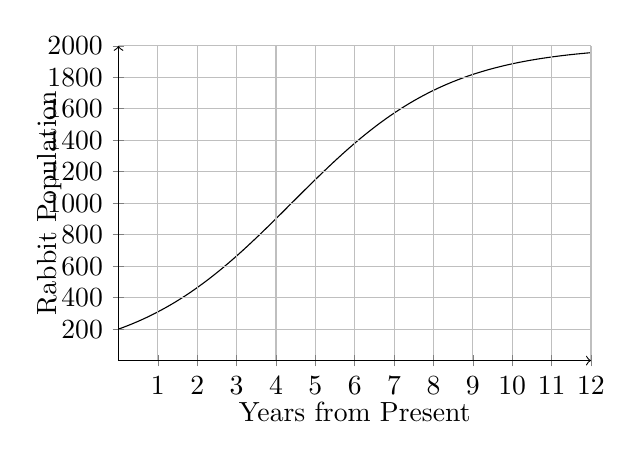
\begin{tikzpicture}
\begin{axis}[
    xmin=0, xmax=12,
    ymin=0, ymax=2000,
    axis lines=center,
    axis on top=true,
    domain=0:1,
    x=0.5cm,
    y=0.002cm,
    xtick={0,1,...,20},
    xticklabels={0,1,...,20},
    ytick={0,200,...,2000},
    yticklabels={0,200,...,2000},
    axis lines=middle,
    axis line style={->},
    x label style={at={(axis description cs:0.5,-0.1)},anchor=north},
    y label style={at={(axis description cs:-0.1,.5)},rotate=90,anchor=south},
    xlabel={Years from Present},
    ylabel={Rabbit Population},
    grid=major
    ]
	\addplot[samples=100,domain=0:12] {2000/(1+9*e^(-0.5*x))};
\end{axis}
\end{tikzpicture}
\end{center}
Note that according to the model, the rabbit population will level out near the carrying capacity in about 12 years.

\item In 8 years, the population is predicted to be approximately
\begin{align*}
P_8 &= \dfrac{2000}{1+9e^{-0.5(8)}}\\
&= \dfrac{2000}{1+9(0.01832)}\\
&= \dfrac{2000}{1.1648}
&= \boxed{1717 \textrm{ rabbits}}
\end{align*}

\item We'll use the calculator for this: graph the model and the horizontal line at 1000, and find their intersection:
\begin{center}
\begin{tabular}{c c c}
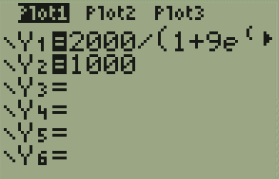
\includegraphics[height=0.9in]{RabbitGraph1}
& 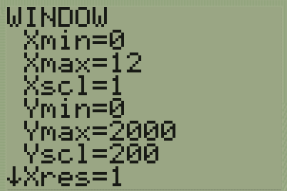
\includegraphics[height=0.9in]{RabbitGraph2}
& 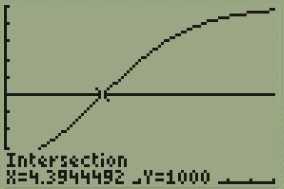
\includegraphics[height=0.9in]{RabbitGraph3}
\end{tabular}
\end{center}

The intersection is at $x=4.394$, so the population is expected to reach 1000 rabbits after about $\boxed{4.4 \textrm{ years}}$
\end{enumerate}
\end{example}
\pagebreak

\subsection{Logistic Regression}
As before, it is unlikely that we will know at the beginning of a study what the growth rate is; it's more likely that we'll have data and need to build a model to fit.  We'll use a graphing calculator to do this; although Excel can do it, it is not built-in to the menus that we have used before, and the process is very involved, so we will not include that in this chapter.

\begin{example}[https://www.youtube.com/watch?v=7gXNhLY1Yyc&list=PLfmpjsIzhztutjEb8Pg5OBOlI1p80yVoy&index=15]{Logistic Regression}
\marginnote{
\includegraphics[width=1.5in]{nycgray}}
Build a logistic population model for New York City using the population data below.
\begin{center}
\begin{tabular}{c c}
\textbf{Year} & \textbf{Population (millions)}\\
\hline
& \\
1900 & 3.44\\
1910 & 4.77\\
1920 & 5.62\\ 
1930 & 6.93\\
1940 & 7.45\\
1950 & 7.89\\
1960 & 7.78\\
1970 & 7.89\\
\end{tabular}
\end{center}

\sol
First, enter the data (setting 1900 as year 0) and draw a scatterplot to get a visual sense of it:
\begin{center}
\begin{tabular}{c c}
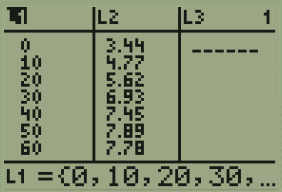
\includegraphics[height=1.2in]{NYCLogistic1}
& 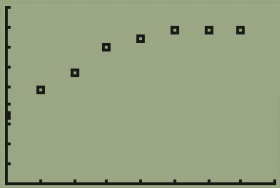
\includegraphics[height=1.2in]{NYCLogistic2}
\end{tabular}
\end{center}

To get the regression equation, enter the \calcbutton{STAT} \texttt{CALC} menu, then select \texttt{B: Logistic} near the bottom of the list.  Once again, since we entered time in the first data column and population in the second, we can leave the default options unchanged.
\begin{center}
\begin{tabular}{c c}
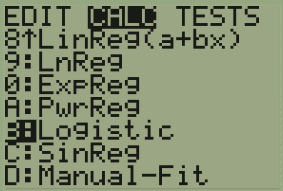
\includegraphics[height=1.2in]{NYCLogistic3}
& 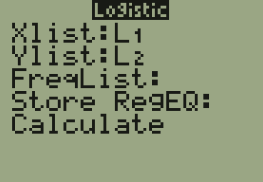
\includegraphics[height=1.2in]{NYCLogistic4}
\end{tabular}
\end{center} 

The results are shown below; the graph on the right shows how the model tracks the data.
\begin{center}
\begin{tabular}{c c}
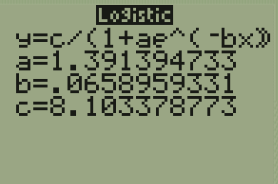
\includegraphics[height=1.2in]{NYCLogistic5}
& 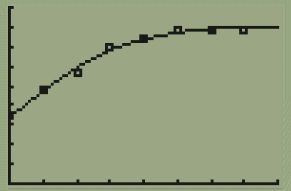
\includegraphics[height=1.2in]{NYCLogistic6}
\end{tabular}
\end{center}
The model is \[\boxed{P_t = \dfrac{8.1}{1+1.39e^{-0.066t}}}\]
Notice on the graph above how this model accounts for the leveling off of the population near the end.
\end{example}